\documentclass[12pt]{article}
\usepackage{nott-titlepage}
\usepackage{graphicx}
\usepackage{float}
\usepackage{amsmath}
\usepackage{hyperref}
% https://tex.stackexchange.com/questions/32598/force-latex-image-to-appear-in-the-section-in-which-its-declared
\usepackage[section]{placeins}

\title{EEEE3112 Coursework 2 Inverter Design}
\author{Tan Hong Kai}
\date{May 13, 2024}
\studentid{20386501}
\module{EEEE3112 Power Electronic Applications and Control}
\department{Department of Electrical and Electronics}

\begin{document}
\maketitle

\section{Introduction}

This coursework explores the design of DC to AC inverter.
The inverter is a single-phase grid connected inverter facing a solar power network.
The design specification of the inverter is shown in table \ref{tab:design-spec}.

\begin{table}[H]
    \caption{Design Specification of the Inverter}
    \label{tab:design-spec}
    \centering{}
    \begin{tabular}{l l  l}
        \hline
        Specification/Term                  & Symbol      & Value  \\
        \hline
        DC Voltage                          & $V_{DC}$    & 600 V  \\
        AC RMS Voltage                      & $V_{AC}$    & 240 V  \\
        AC Current Ripple (peak-peak)       & $\Delta{I}$ & 0.5 A  \\
        Rated Power                         & $P$         & 3 kW   \\
        Inverter Switching Frequency        & $f_{sw}$    & 20 kHz \\
        Loss in the Inductor at Rated Power & $P_{LOSS}$  & 1\%P W \\
        Reactive Power                      & $Q_{AC}$    & 0 W    \\
        \hline
    \end{tabular}
\end{table}

In this coursework, all the calculations are done in a Matlab live script.
Furthermore, the live script also contains the code for the control design and analysis.
Using a live script allows for quick calculations of values if any changes were made and the built-in markup makes the code organize.
Once the values for the inverter are calculated, the inverter is then modelled and simulated in PLECS to evaluate the performance.

\section{Inductor Design}

The first part of an inverter design is designing the inductor.
The inductor sits between the inverter and the AC grid.
It acts as a filter to the high frequency of the inverter.
Furthermore, the inductor acts as a load with low losses to allow for power transfer.

The main components that effects the inductor design is the AC current ripple $\Delta{I}$.
However, there are other components such as the switching period and DC input voltage which are usually fixed.
Formula \ref{eq:inductor} shows how the inductor size is calculated.
Where $T_{s}$ is the switching period $\frac{1}{f_{sw}}$.

\begin{equation} \label{eq:inductor}
    L = \frac{T_{s} V_{DC}}{8 \Delta{I}} = \frac{0.00005 * 600}{8 * 0.5} = 7.5 mH
\end{equation}

Inductors are not ideal and has some resistance in it.
In this coursework, the resistance of the inductor contributes to 1\% of the rated power.
It can be calculated using the power loss equation:

\begin{equation}
    \begin{aligned}
        P_{LOSS} & = I^{2} R                \\
        R        & = \frac{P_{LOSS}}{I^{2}}
    \end{aligned}
\end{equation}

Where:

\begin{equation}
    \begin{aligned}
        I       & = \frac{\sqrt{P^{2} + Q_{AC}^{2}}}{V_{AC}} = \frac{\sqrt{3000^{2} + 0^{2}}}{240} = 12.5 A \\
        \varphi & = -\arctan(\frac{Q_{AC}}{P_{AC}}) = -\arctan(0) = 0^{\circ{}}
    \end{aligned}
\end{equation}

Therefore:

\begin{equation}
    R = \frac{0.01 * 3000}{12.5^{2}} = 0.192 \Omega
\end{equation}

\section{Inverter Voltage}

The power delivered by the inverter to the grid is based on the inverter voltage $V_{INV}$.
Inverter voltage is mainly effected by the current delivered $I$ and inductor impedance $Z$.
The inverter voltage can be calculated using formula \ref{eq:v-inv}.
Note that all the values are calculated in the phasor representation.

\begin{equation} \label{eq:v-inv}
    \begin{aligned}
        \dot{Z}       & = \omega{L}j = 2 * \pi * 50 * 7.5m * j = 2.356j \Omega                   \\
        \dot{V}_{INV} & = \dot{I} \dot{Z} + \dot{V}_{AC} = 12.5 * 2.356j + 240 = 240 + 29.452j V
    \end{aligned}
\end{equation}

The time domain equation can be obtained by converting it from the phasor representation.

\begin{equation}
    \begin{aligned}
        V_{INV}       & = \sqrt{240^2 + 29.452^2} = 241.800 V                                                  \\
        \hat{V}_{INV} & = V_{INV} * \sqrt(2) = 341.957 V                                                       \\
        \gamma        & = \arctan(\frac{29.452}{240}) = 6.996^{\circ{}}                                        \\
        V_{INV}(t)    & = \hat{V}_{INV} \sin(\omega{t} + \gamma{}) = 341.957 \sin(\omega{t} + 6.996^{\circ{}})
    \end{aligned}
\end{equation}

\section{Average Time Model}
\label{sec:avg-time-model}

An average time model of the inverter is design.
In this model, the inverter is modelled as a controllable voltage source.
The inverter is then connected to the grid with the inductor calculated in between.
Measurements of the inverter current and AC grid voltage is taken to calculate the power output.
Figure \ref{fig:avg-time-waveform} shows the output wave forms of the inverter and the average output power.

\begin{figure}[H]
    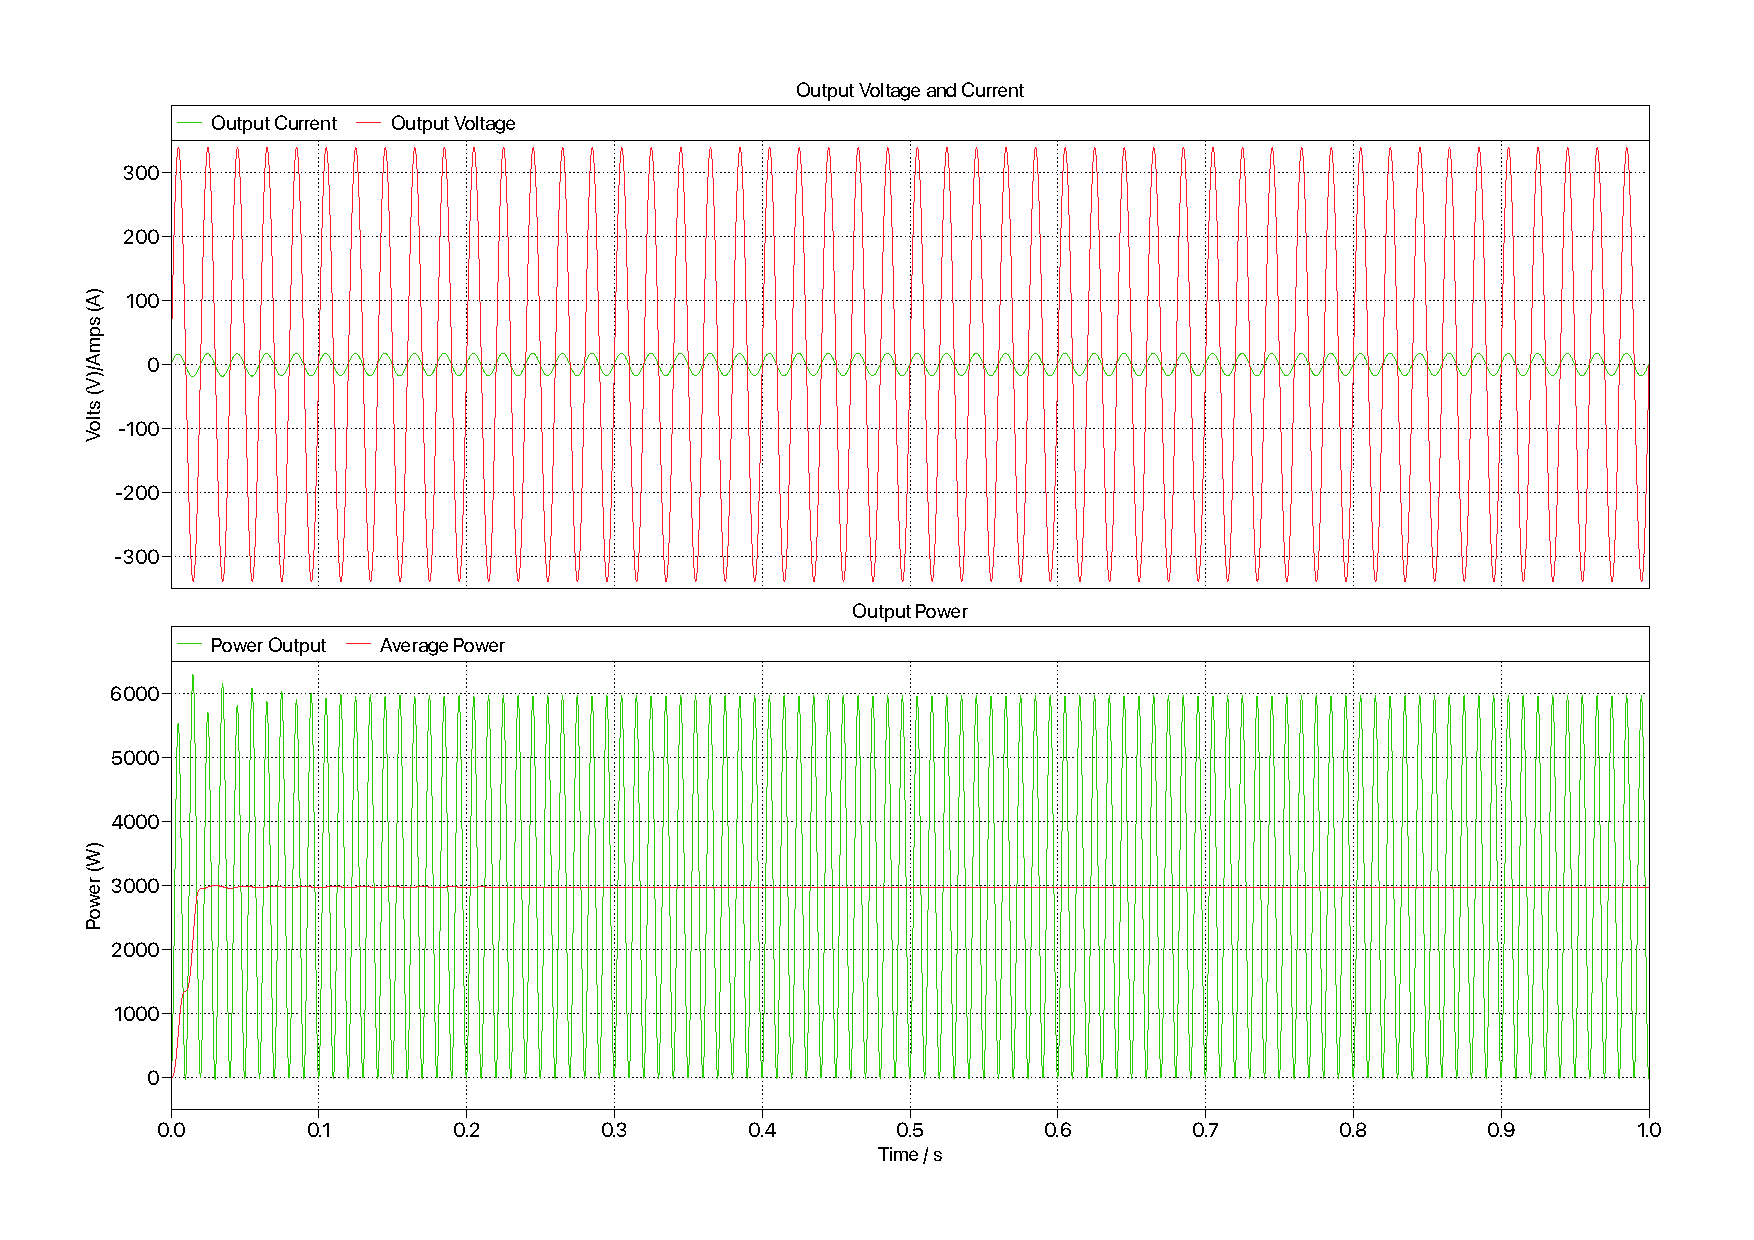
\includegraphics[width=\textwidth]{img/Average Time Power.pdf}
    \caption{Output Waveforms of the Average Time Model Inverter}
    \label{fig:avg-time-waveform}
\end{figure}

\begin{figure}[H]
    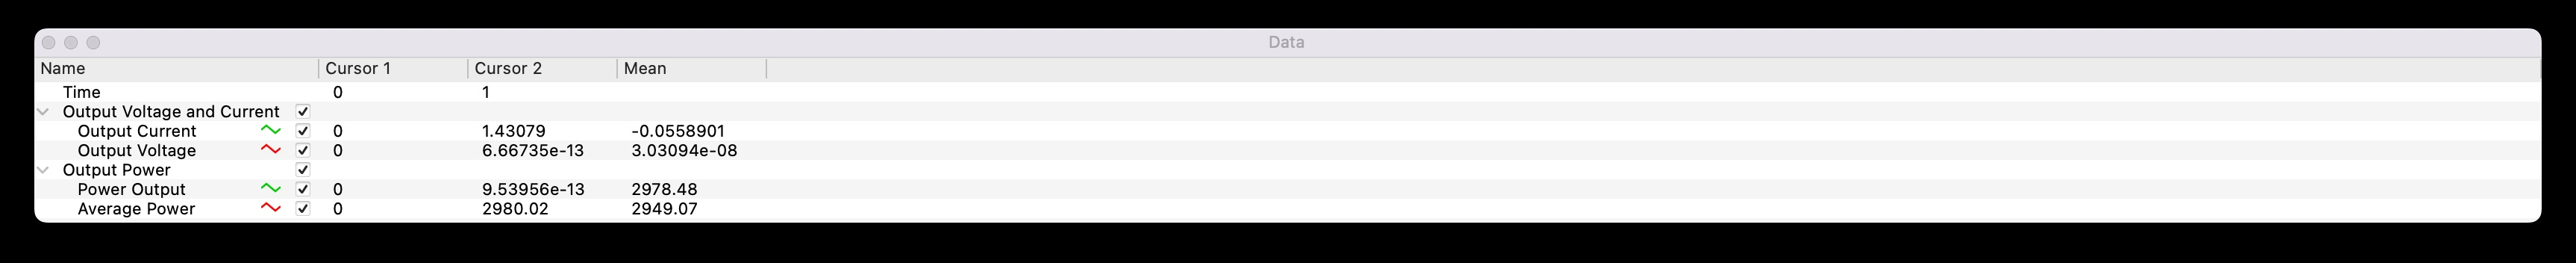
\includegraphics[width=\textwidth]{img/Average Timer Power Cursor.jpg}
    \caption{Measurements from the Average Time Model Waveform}
    \label{fig:avg-time-cursor}
\end{figure}

The waveforms show that the power output of the inverter matches with the calculated values.
The average power of the inverter is around 2980 W.
This is close to the expected power of $3000 - 1\% * 3000 = 3000 - 30 = 2970$ W.
The difference is due to the precision of the calculated and input values to PLECS.

\section{Switching Model}

A new model is created using a full bridge converter.
This model includes the switching devices (IGBT with diode), DC voltage source and the PWM modulator.
The output of the converter is connected to the grid with the inductor in the middle.

An IGBT is chosen due to the high power application of the inverter.
Furthermore, a freewheeling diode is added to allow for bidirectional current flow.
The IGBT is controlled by the PWM output $G_{B1}$ and $G_{B2}$.

The PWM modulator consists of a comparator for each output.
The negative rail of the comparators are connected to a triangular wave with 20 kHz frequency.
The positive rail of the $G_{B1}$ comparator is connected to $m_1(t)$ while $G_{B2}$ is connected to $m_2(t)$.
Where:

\begin{equation}
    \begin{aligned}
        m_1(t) & = 0.5 + \frac{V_{INV}(t)}{2 V_{DC}} \\
        m_2(t) & = 0.5 - \frac{V_{INV}(t)}{2 V_{DC}} \\
    \end{aligned}
\end{equation}

\begin{figure}
    \centering{}
    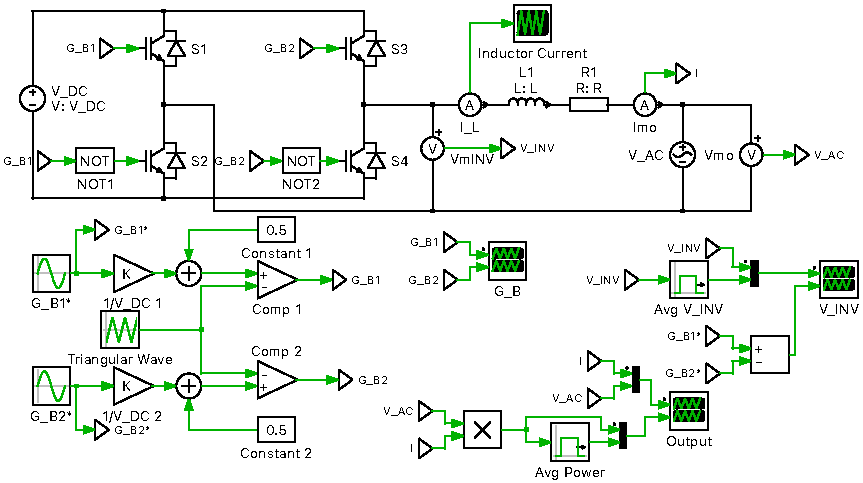
\includegraphics[width=\textwidth, height=0.4\textheight, keepaspectratio]{img/Switching Model.pdf}
    \caption{PLECS Model for the Switching Model}
    \label{fig:switching-model}
\end{figure}

In figure \ref{fig:switching-waveform} and \ref{fig:switching-cursor}, the output current and voltage is measured, and the power is calculated.
The calculated average power output is the same as the one in the \hyperref[sec:avg-time-model]{average time model}.

\begin{figure}
    \centering{}
    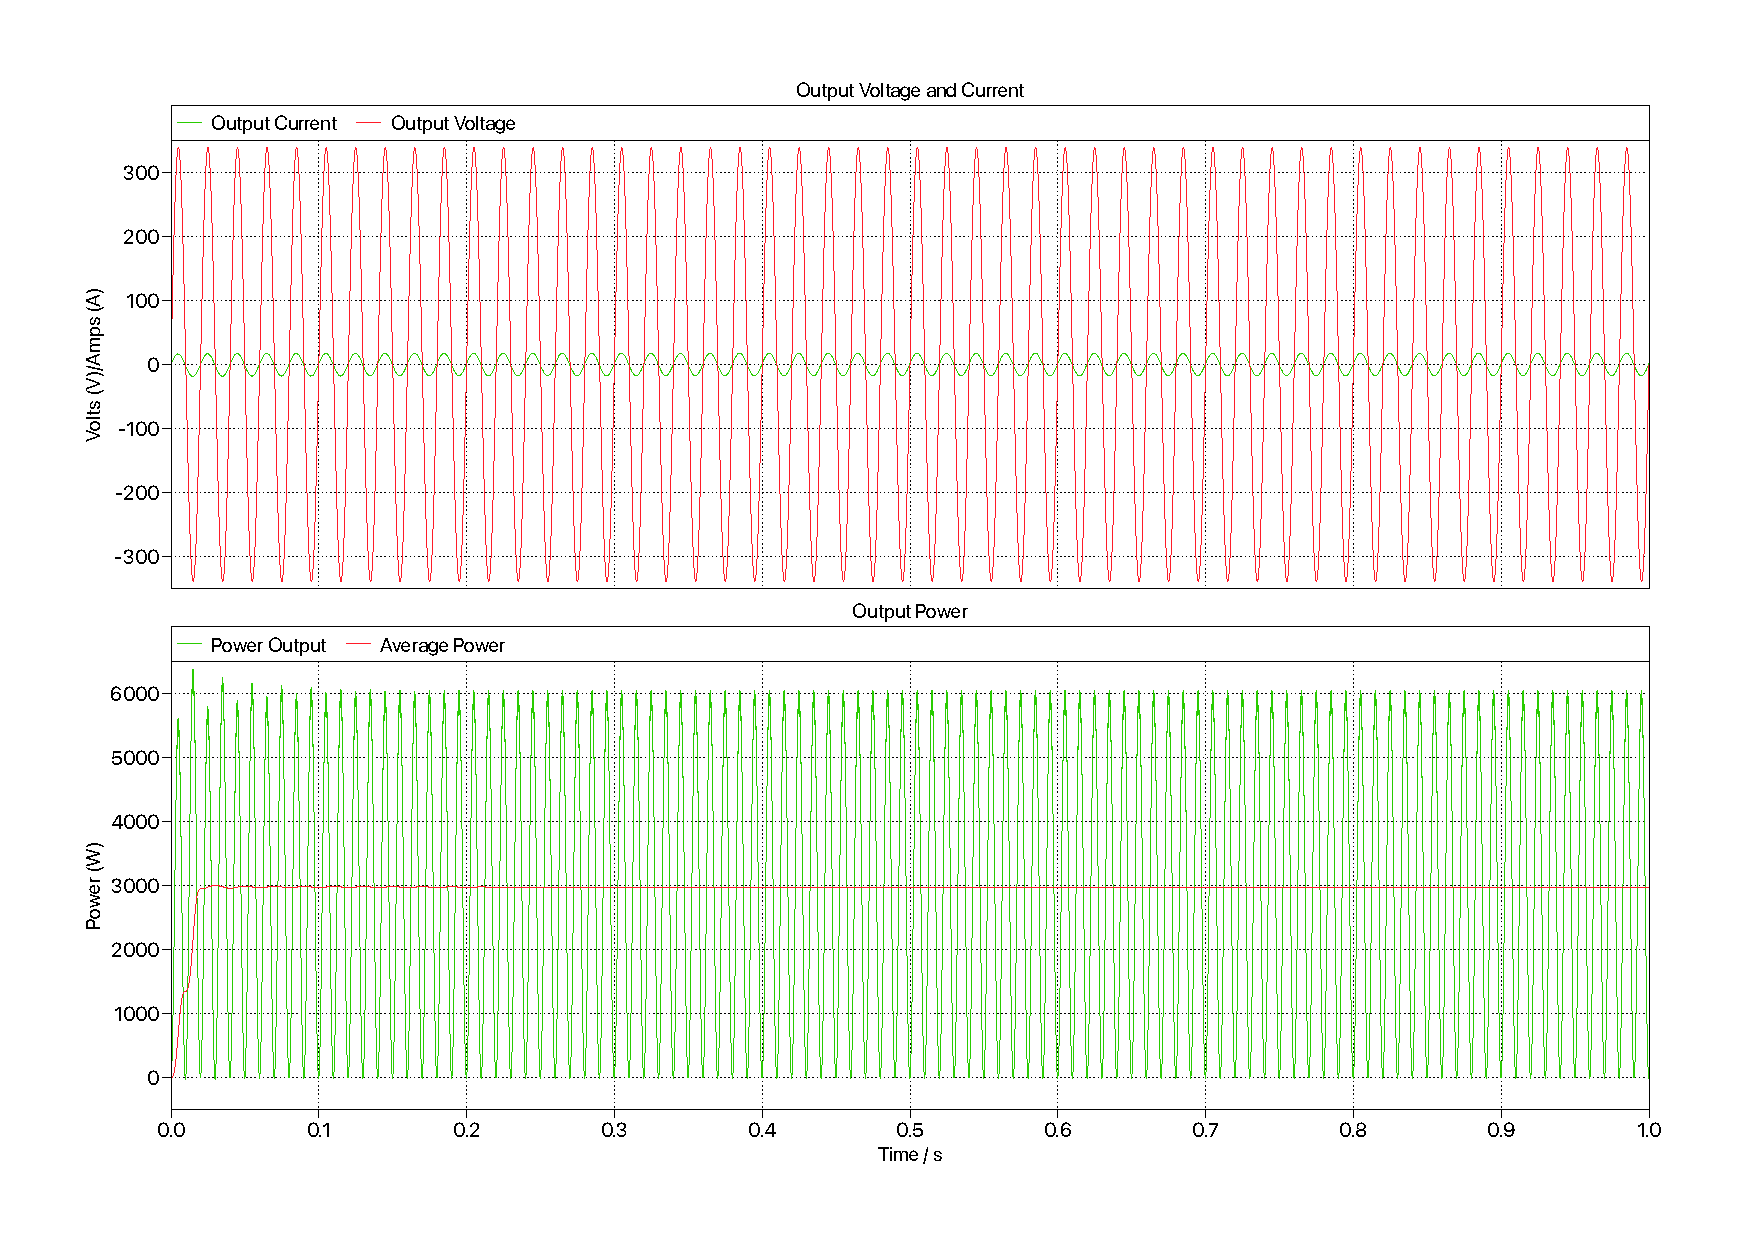
\includegraphics[width=\textwidth, height=0.4\textheight, keepaspectratio]{img/Switching Power.pdf}
    \caption{Output Waveforms of the Switching Model Inverter}
    \label{fig:switching-waveform}
\end{figure}

\begin{figure}
    \centering{}
    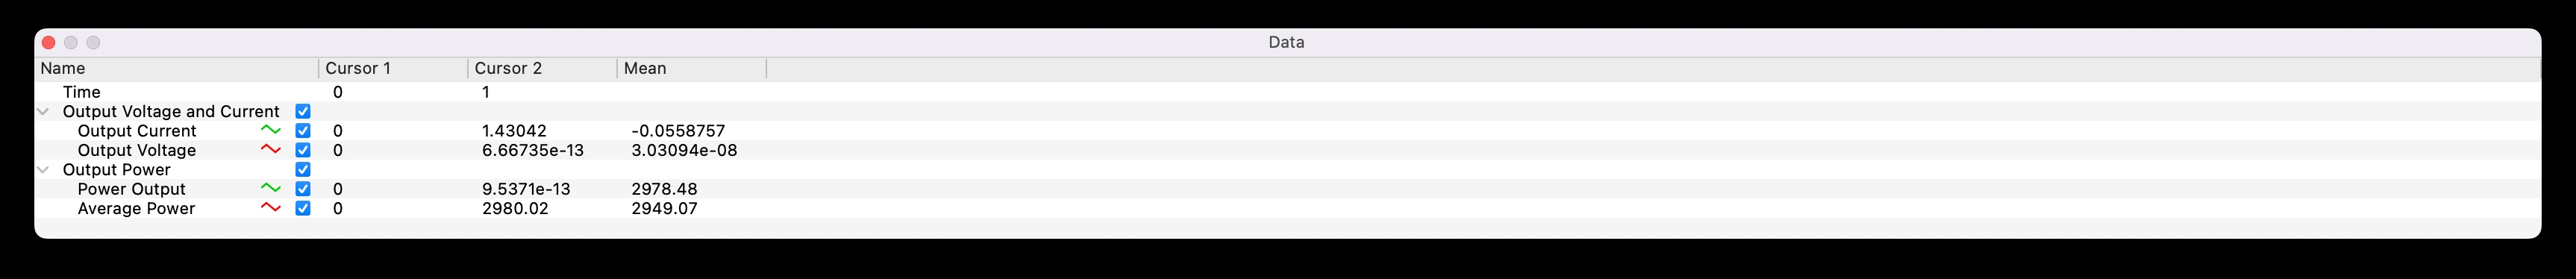
\includegraphics[width=\textwidth, height=0.4\textheight, keepaspectratio]{img/Switching Power Cursor.jpg}
    \caption{Measurements from the Switching Model Waveform}
    \label{fig:switching-cursor}
\end{figure}

Other than output power, the inverter voltage is measured and compared to the voltage demand.
The inverter voltage PWM wave-form is averaged over the switching frequency to show the low frequency component.
In figure \ref{fig:switching-inverter-voltage}, the wave-forms shows that the inverter voltage is able to keep up with the voltage demand generated by the PWM modulator.

To further analyse the inverter voltage, a Fourier analysis is performed.
The Fourier spectrum \ref{fig:switching-fourier} shows that the PWM output have two main frequency spikes.
The first spike occurs at around 0 Hz.
This is due to the low frequency component of the output at 50 Hz.
The value is not at 50 Hz due to the resolution of the frequency axis when sampling for FFT.
The second frequency spike occurs at about 40 kHz.
This is 2 times of the switching frequency.
The inverter output voltage consists of the combination of two half bridges switching at 20 kHz.
When the output of both half bridge combined the 20 kHz harmonics add up to 40 kHz causing the frequency spike at the Fourier analysis.

\begin{figure}
    \centering{}
    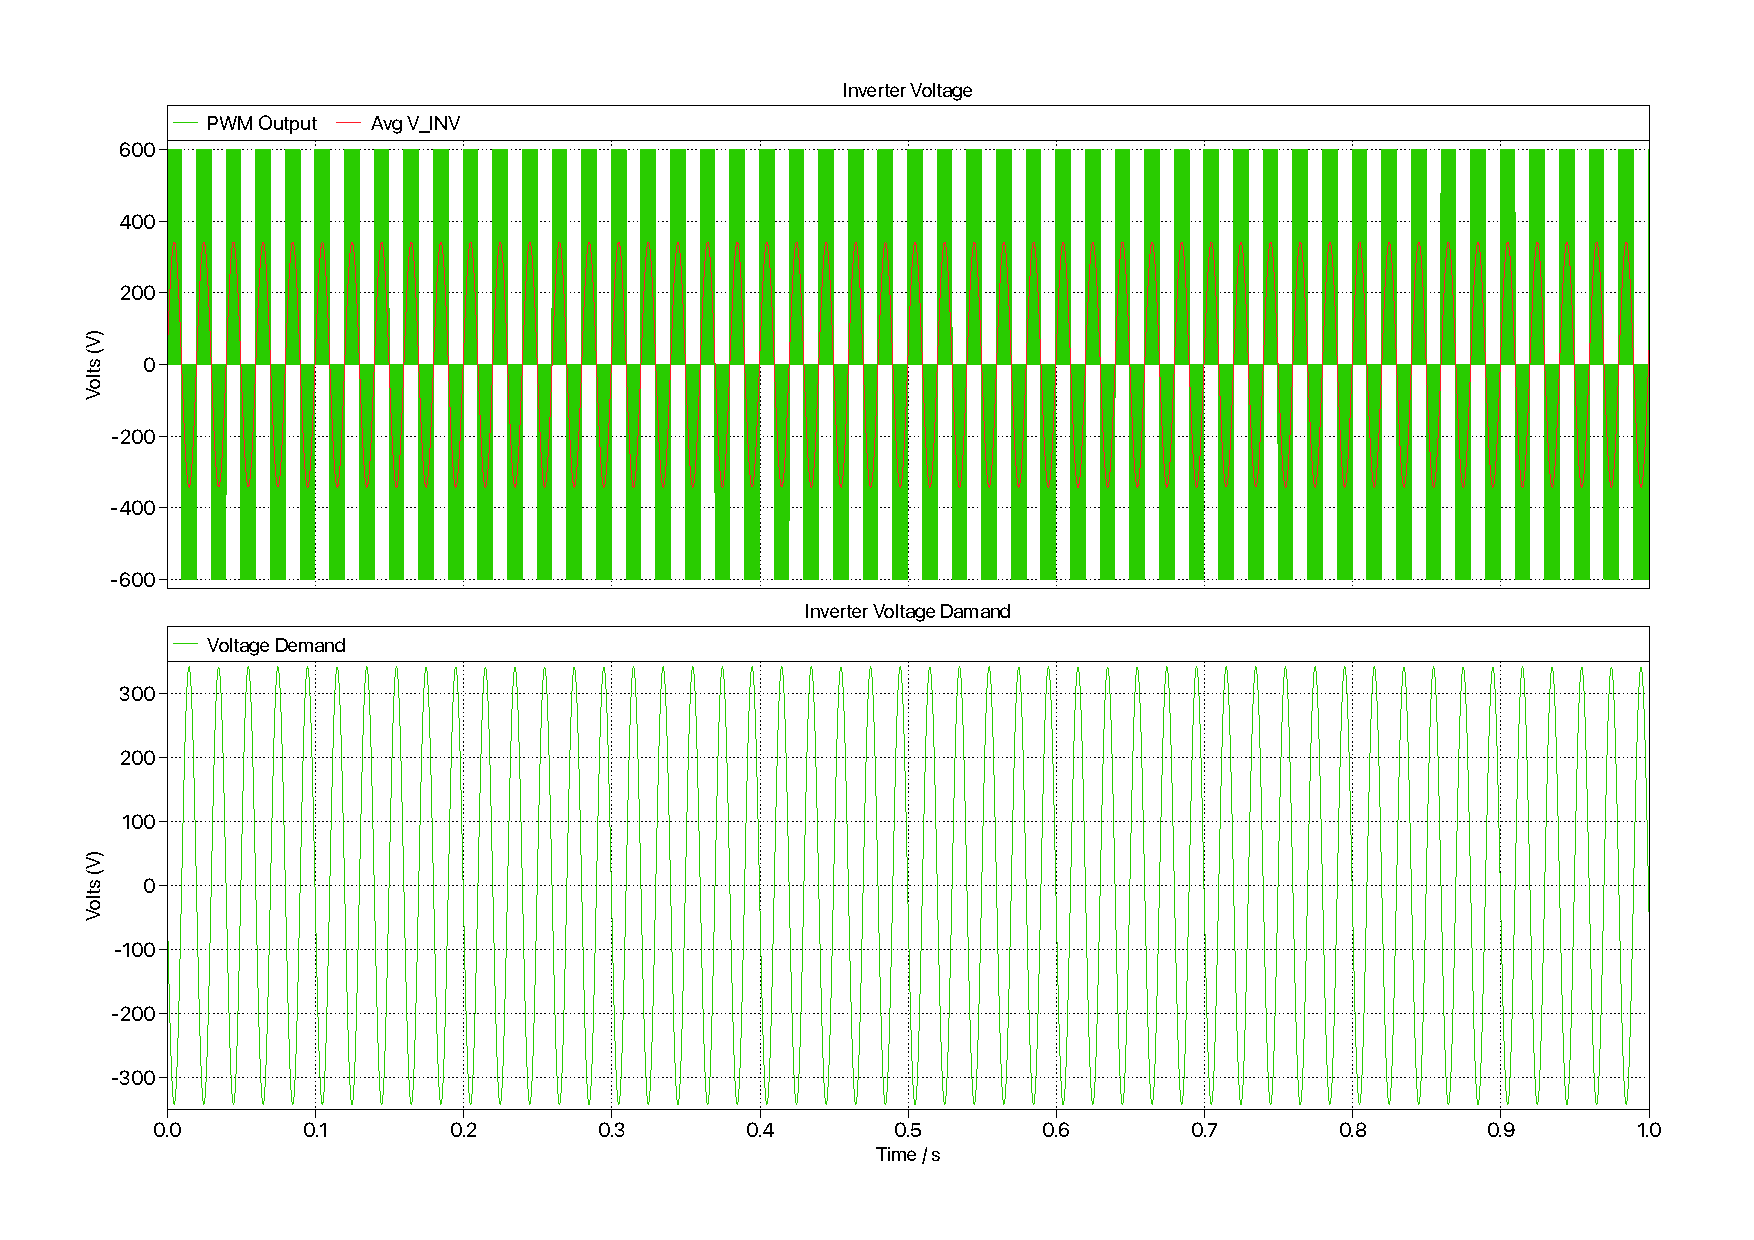
\includegraphics[width=\textwidth, height=0.4\textheight, keepaspectratio]{img/Switching Inverter Voltage.pdf}
    \caption{Output Waveforms of the Inverter Voltage}
    \label{fig:switching-inverter-voltage}
\end{figure}

\begin{figure}
    \centering{}
    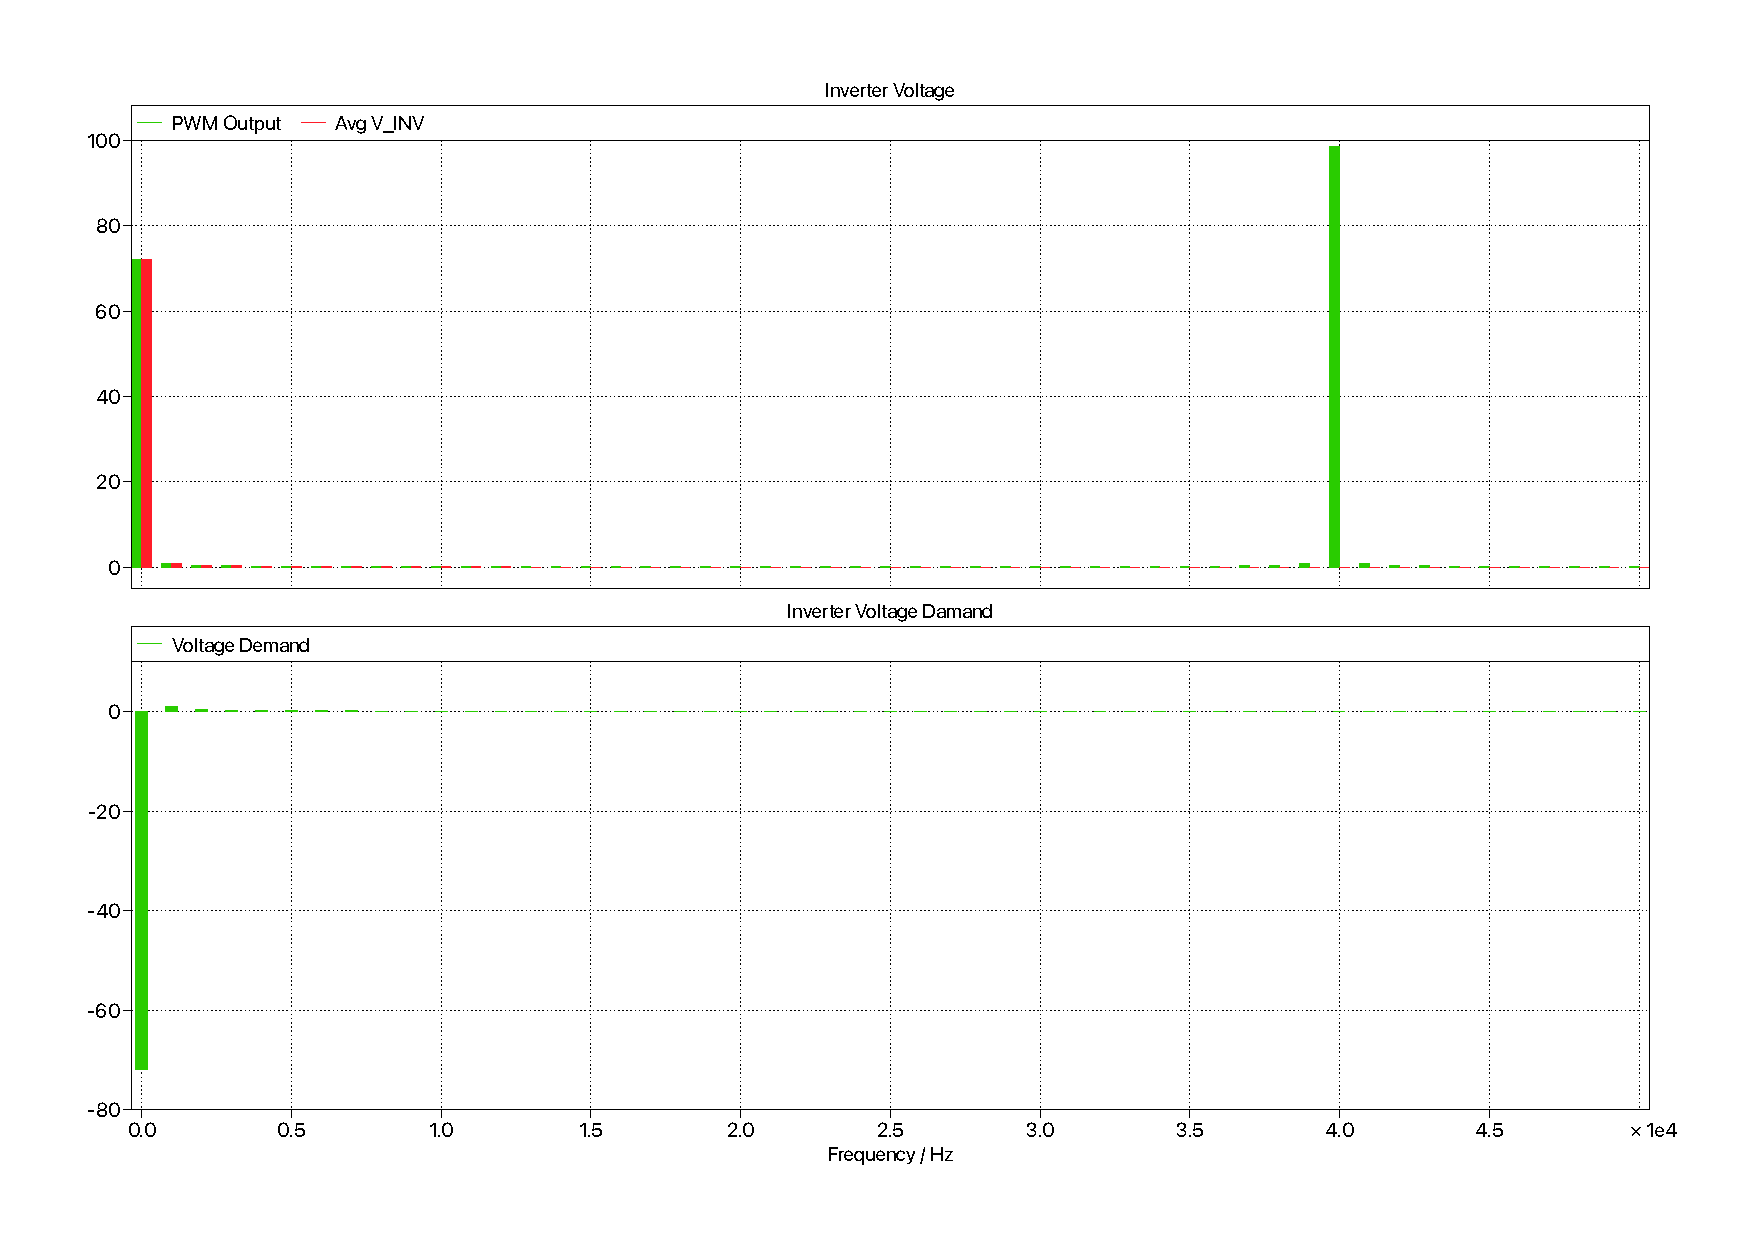
\includegraphics[width=\textwidth, height=0.4\textheight, keepaspectratio]{img/Switching Demand FFT.pdf}
    \caption{Fourier Analysis of the Inverter Voltage}
    \label{fig:switching-fourier}
\end{figure}

The inductor ripple is also considered in the simulation.
Figure \ref{fig:switching-current-ripple} shows the inductor current ripple graph.
From the simulation, the peak to peak current ripple is measured to be 0.491 A which is within the 0.5 A requirement.

\begin{figure}
    \centering{}
    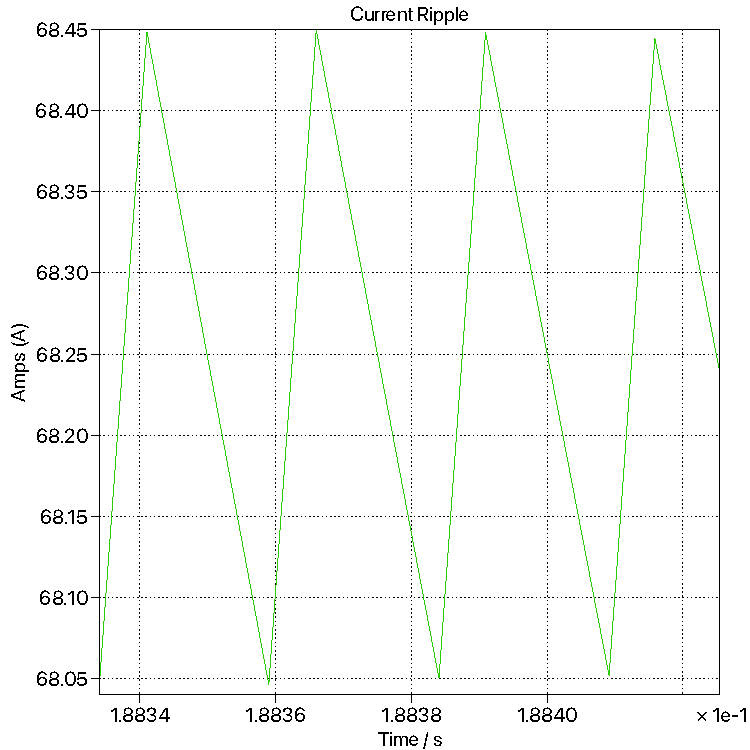
\includegraphics[width=\textwidth, height=0.4\textheight, keepaspectratio]{img/Switching Current Ripple.pdf}
    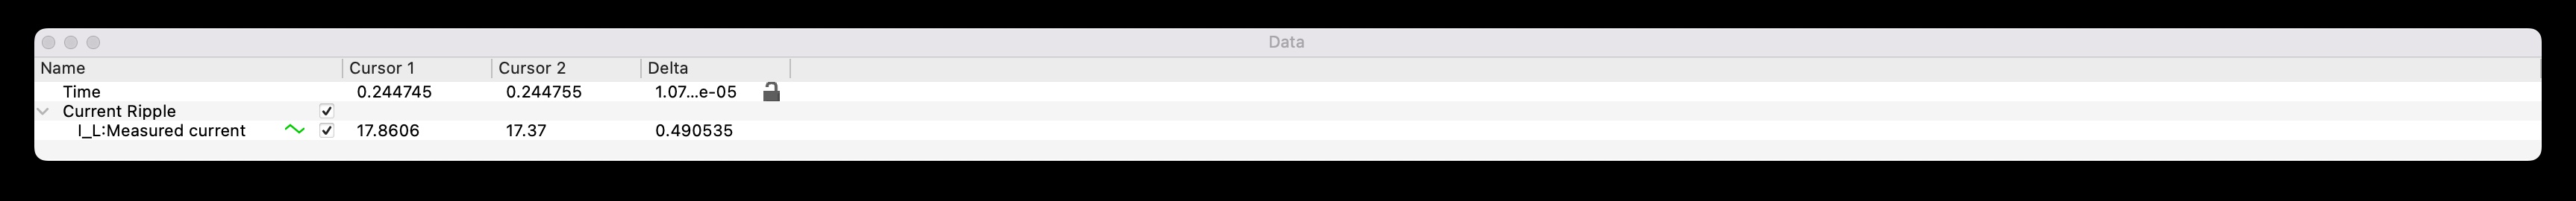
\includegraphics[width=\textwidth, height=0.4\textheight, keepaspectratio]{img/Switching Current Ripple Cursor.jpg}
    \caption{Inductor Current Ripple}
    \label{fig:switching-current-ripple}
\end{figure}

\section{Transfer Function Model}

\section{Continuous Current Control Model}

\section{Discrete Current Control Model}

\section{Conclusion}

\end{document}
